\chapter{Methodology}
\label{ch:method}

This chapter describes the engineering pipeline and methodology employed in constructing and training our multi-agent soccer agents. Our work is comprised of several different components which we will define throughout this chapter: the physical constraints of the simulation environment; the mathematical definition of observation and action spaces; the design of the custom reward shaping wrapper; and the hyperparameters selected to conduct policy training.

In terms of the environment, we begin by defining MuJoCo Soccer 2v2 and its associated physical limits and state dynamics. Next, we formally define the observation space $\mathcal{O}$ available to each agent $i \in \{1, \dots, n\}$, as well as the continuous action space $\mathcal{A}$ governing how those agents can move. We also provide a walkthrough of our custom reward shaping wrapper $\mathcal{F}: r_t \rightarrow r'_t$, which transforms sparse, goal-based rewards into dense and physically meaningful feedback signals that provide value to agents during initial training. Finally, the last section presents the hyperparameter settings $\Theta$ used across the three training algorithms, along with a rationale for the design decisions made to ensure stability and efficient convergence on a single Colab GPU.

% ================================================================
\section{Multi-Agent System Architecture}
\label{sec:method_design}
% ================================================================

The multi-agent soccer pipeline is composed of four main phases:

\begin{enumerate}
    \item \textbf{Environment Wrapper Architecture:} Standardizing the raw MuJoCo multi-agent simulator by utilizing Shimmy and PettingZoo wrappers. This phase ensures that each agent $i \in \{1, \dots, n\}$ receives the same environmental observations $o_i \in \mathcal{O}$ and actions $a_i \in \mathcal{A}$, providing a consistent and reproducible foundation for all future training phases.

    \item \textbf{Custom Reward Wrapper Design:} Building a custom class $\mathcal{F}: r_t \rightarrow r'_t$ to calculate dense intermediate rewards based on continuous physical coordinates $(x_t, y_t)$, providing agents with meaningful feedback throughout the entire episode instead of solely at the goal-scoring moment. Agents will learn how to move and operate meaningfully from the beginning of the training process.

    \item \textbf{Cooperative Shared-Policy Training:} Using PPO to optimize the agent parameters $\theta_i = \theta \; \forall i \in \{1, \dots, n\}$ while sharing weights among all agents on a team, allowing all agents to use a single policy $\pi_\theta$ to reduce the total number of trainable parameters. This encourages cooperative behavior between teammates during training with only one Colab GPU.

    \item \textbf{Offline Spatial Analytics:} Performing post-training evaluations to generate coordinate trajectories $(x_t, y_t)$ of each agent and compiling 2D spatial hexbin heatmaps, teammate distance distributions $d(s_i, s_j)$, and possession statistics. These metrics provide a quantitative measure of agent performance.
\end{enumerate}

\begin{figure}[!ht]
    \centering
    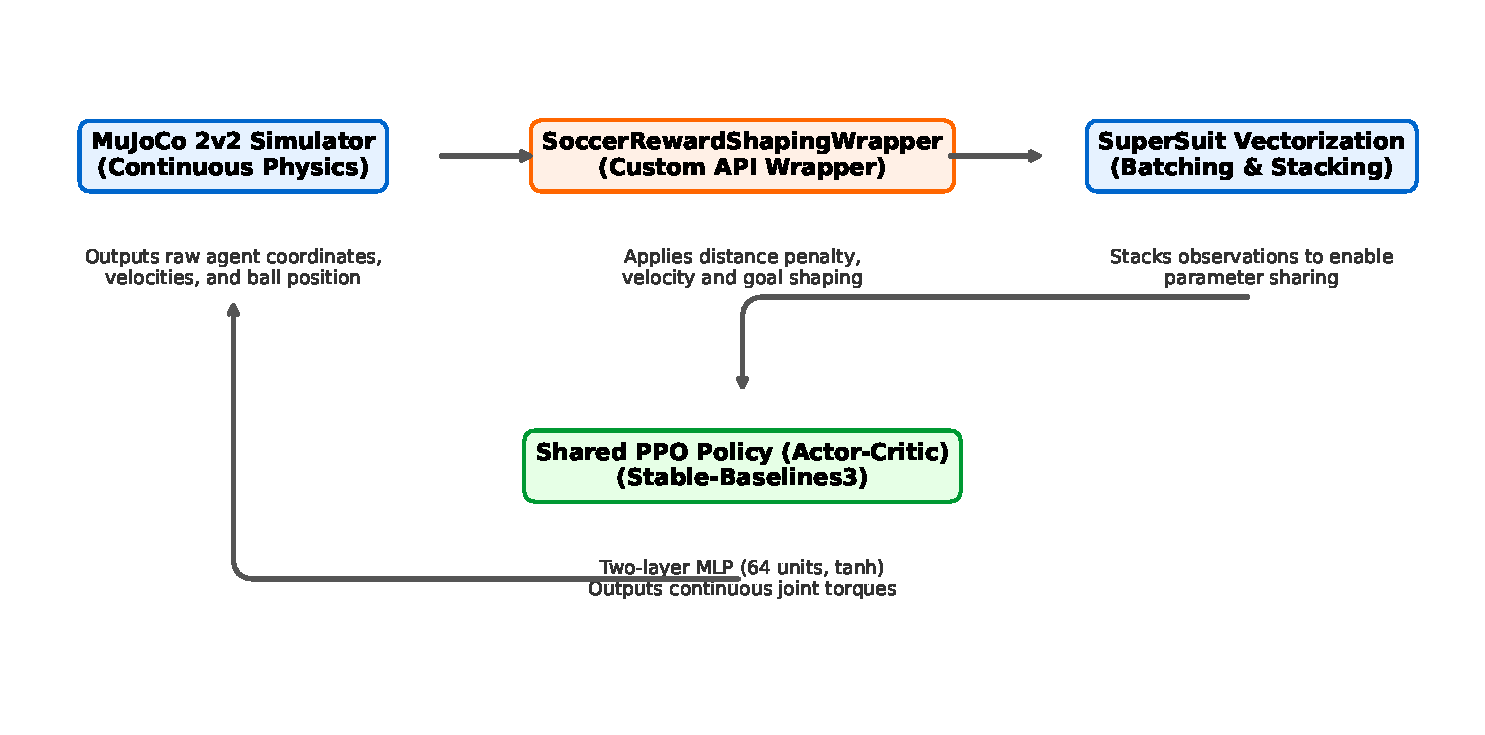
\includegraphics[width=0.95\textwidth]{figures/system_architecture.pdf}
    \caption{System architecture of the multi-agent reinforcement learning soccer simulator pipeline.}
    \label{fig:system_architecture}
\end{figure}
% ================================================================
\section{MuJoCo Soccer 2v2 Simulation Environment}
\label{sec:method_soccer_env}
% ================================================================

Our setup uses the multi-agent soccer environment from the DeepMind Control Suite~\citep{tassa2020dmcontrol}, integrated via the Shimmy library~\citep{shimmy2022} and conforming to the PettingZoo Parallel API standard~\citep{terry2021pettingzoo}. The simulation implements a continuous 3D physics sandbox representing a soccer pitch.

\subsection{Physical and Kinematic Specifications}
Four physical agents make up the simulated environment and are split into two teams of two members each: the attacking Team Red and the defending Team Blue. The physical agents interact with each other using the MuJoCo physics engine, which models dynamics such as solid-body collisions, coefficient of static friction $\mu$, linear momentum $\mathbf{p} = m\mathbf{v}$, and rotational momentum $\mathbf{L} = I\boldsymbol{\omega}$ due to its joint constraints. The two-dimensional coordinate system describes the size of the pitch using an $X$-axis with the range $[-12.0, +12.0]$ for length and a $Y$-axis with range $[-8.0, +8.0]$ for width, yielding a total playing area of $24.0 \times 16.0$ units. This configuration provides a realistic and controlled environment to study how individual agents $i \in \{1, \dots, 4\}$ can demonstrate competitive behavior in multi-agent scenarios.

\subsection{State Observation and Action Spaces}
Handling continuous physical interactions requires structured egocentric representations:
\begin{itemize}
    \item \textbf{Observation Space (Dictionary-based))}: Each agent perceives the environment through a local egocentric observation dictionary containing:

    \begin{itemize}
    \item \textbf{ball\_ego\_position:} A $2$D vector $(x, y)$ representing the relative coordinates of the ball in the agent's own coordinate frame. This vector is updated at each timestep $t$ relative to where the agent currently resides on the field, always providing information on where the ball is located relative to the agent's current position and orientation.

    \item \textbf{stats\_vel\_to\_ball:} A scalar value indicating the agent's speed in the direction of the ball. A positive value means that the agent is getting closer to the ball, while a negative value means that the agent is moving further away from the ball. This signal can therefore be used to shape the agent's rewards during training.

    \item \textbf{stats\_vel\_ball\_to\_goal:} A scalar value that indicates the direction of the ball with respect to the location of the opponent's goal mouth and how fast the ball is progressing toward the goal.
    \end{itemize}
    \item \textbf{Action Space (Continuous Torques)}: The actions that can be taken are determined by the control inputs, where each input represents the amount of normalized torque applied to each of the agents’ joint actuators. The agents will have joint actuators for each of their leg and torso joints (e.g. the hip and ankle and also knee) so the policy can create running and turning and kicking motions.
\end{itemize}

\begin{figure}[!ht]
    \centering
    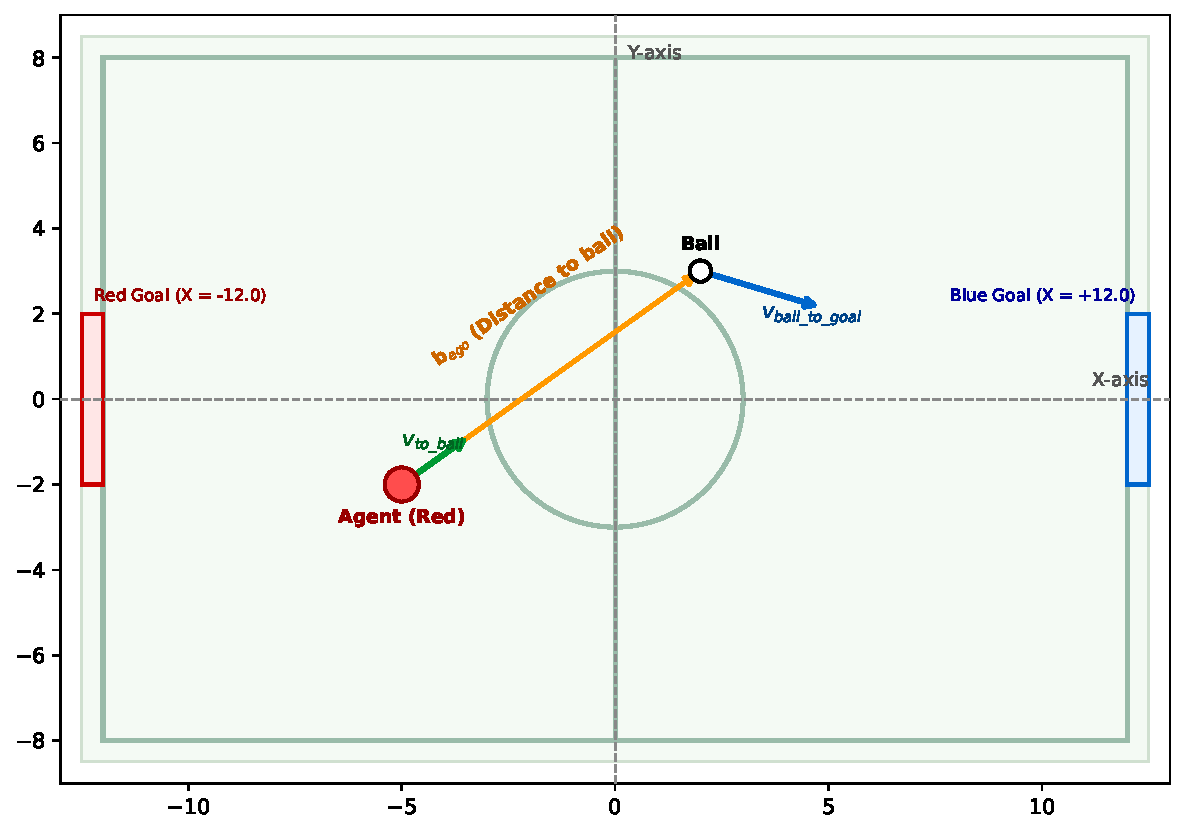
\includegraphics[width=0.90\textwidth]{figures/pitch_coordinates.pdf}
    \caption{Visual representation of the 3D soccer pitch coordinate axes and egocentric agent observations.}
    \label{fig:pitch_coordinates}
\end{figure}

% ================================================================
\section{Proximal Policy Optimisation (PPO) with Shared Policies}
\label{sec:method_ppo}
% ================================================================

\subsection{Custom Reward Shaping}
\label{sec:rw_shaping}

Most common rewards in MuJoCo are sparse – agents will only receive rewards when they reach a goal. For example, if an agent explores randomly, there will be very few times it scores and hence, no positive gradients will be found by using any standard policy gradient method. To solve this, we will implement a custom wrapper class \texttt{SoccerRewardShapingWrapper} (which has equal hierarchy to PettingZoo's \texttt{BaseParallelWrapper}) that modifies the step function to include dense intermediate feedback every frame:

\begin{equation}
    r_{\text{shaped}}(a) = r_{\text{env}}(a) + r_{\text{dist}}(a) + r_{\text{vel}}(a) + r_{\text{goal}}(a),
    \label{eq:total_reward}
\end{equation}

where:
\begin{align}
    r_{\text{dist}}(a) &= -0.01 \times \|\mathbf{b}_{\text{ego}}\|_2, \label{eq:dist_penalty} \\
    r_{\text{vel}}(a)  &= 0.10 \times v_{\text{to\_ball}}, \label{eq:vel_reward} \\
    r_{\text{goal}}(a) &= 0.50 \times v_{\text{ball\_to\_goal}}. \label{eq:goal_reward}
\end{align}

Here, $\|\mathbf{b}_{\text{ego}}\|_2$ is the Euclidean distance from the agent to the ball on the pitch plane, $v_{\text{to\_ball}}$ is the agent's velocity vector projected towards the ball, and $v_{\text{ball\_to\_goal}}$ is the ball's velocity vector projected towards the target goal. 

The distance penalty (Eq.~\eqref{eq:dist_penalty}) applies a continuous cost for staying away from the action, preventing passive behaviors. The velocity reward (Eq.~\eqref{eq:vel_reward}) encourages agents to sprint towards the ball. The goal-velocity reward (Eq.~\eqref{eq:goal_reward}) guides the agent to push the ball forward, providing a clean gradient path for scoring.

\subsection{Parameter Sharing and Environment Wrapping}

To share the same actor-critic with multiple teams, we will use parameter sharing among agents of the same team. We want each agent to have the same weights in its policy, rather than having separate and independent networks for each agent. Using a single set of weights reduces the total number of parameters that need to be trained, and allows teammates to learn to work together because they are being trained under the same policy objective.

In order to support our implementation, we use SuperSuit utilities~\citep{supersuit2021} to wrap our PettingZoo environment such that we can stack the observation streams from each individual agent into a single parallel batch of observations. We can then process all agents' observations at the same time via a single Stable-Baselines3 vectorized policy with a single forward pass. Specifically, each timestep we concatenate the observations of all agents into a single batched input tensor and feed that through the shared actor-critic neural network to output the action distributions for each agent. The advantage of processing agents in parallel allows us to simplify the training pipeline and makes it computationally practical to train all agents at once on one Colab GPU without the memory overheads and the computational costs associated with maintaining and updating policy networks for each agent. An example of how to do this in Python can be seen in Listing~\ref{list:env_wrapping}.

\begin{lstlisting}[language=Python, 
    caption={Environment wrapping for parameter sharing.}, 
    label=list:env_wrapping]
env = create_soccer_env(render_mode=None)
env = ss.pettingzoo_env_to_vec_env_v1(env)
env = ss.concat_vec_envs_v1(env, num_vec_envs=1, 
                             num_cpus=1, 
                             base_class='stable_baselines3')
\end{lstlisting}

Using this method, we are able to generate four transition samples (totaling 4 for each agent) during every time step of our simulations, thus greatly increasing the diversity of the sampled transitions for the policy's learning at every update. The use of a shared network allows us to run agents in parallel for each configuration of the simulation, thus providing more opportunities for a wider variety of gradient updates for the policy at every time step, resulting in a significant acceleration of the overall convergence of the training process while also being able to utilize the same number of CPU cycles over the multiple agents as we would if we separated the processing of agent updates during the simulation..

\subsection{PPO Hyperparameters}

We initialize our PPO model using Stable-Baselines3~\citep{raffin2021stablebaselines3} with a \texttt{MultiInputPolicy} to support dictionary observations. Table~\ref{tab:ppo_hyperparams} lists the hyperparameter configurations.

\begin{table}[!ht]
    \centering
    \caption{PPO hyperparameters for MuJoCo Soccer 2v2.}
    \label{tab:ppo_hyperparams}
    \begin{tabular}{lc}
        \toprule
        \textbf{Hyperparameter} & \textbf{Value} \\
        \midrule
        Policy              & MultiInputPolicy \\
        Learning rate       & $3 \times 10^{-4}$ \\
        Batch size          & 4,096 \\
        $n$\_steps          & 4,096 \\
        Entropy coefficient & 0.01 \\
        Total timesteps     & 10,000,000 \\
        Framework           & Stable-Baselines3 \\
        \bottomrule
    \end{tabular}
\end{table}

\subsection{Training Infrastructure}

Using the free cloud platform of Google Colaboratory, we trained all agents using a single T4 GPU instance. Since Colaboratory disconnects automatically after 12 continuous hours of usage, all training progress that is stored in memory is permanently lost during the disconnection event. To mitigate this limitation, checkpoints were set up using a custom \texttt{CheckpointCallback} function to automatically save the weights of the current policy to Google Drive every 200,000 environment steps.

This strategy allowed us to safely continue training across multiple separate sessions. At the start of each new session, the most recent checkpoint would be obtained from Google Drive and the training would then continue from where it had previously stopped rather than starting over from scratch. By utilizing this method it allowed us to complete our full training duration despite the limitations of using this platform, without needing access to dedicated high-performance computing.

To ensure that the maximum possible amount of progress would be recoverable, the 200,000 environment step saving interval was purposely selected to be a balance between the frequency of checkpoints and storage efficiency. Therefore, if an unexpected disconnection were to occur, the maximum possible amount of training progress lost would still be in a recoverable range.

% ================================================================
\section{Ethical Considerations}
\label{sec:ethics}
% ================================================================

In this project we employ simulated environments and publicly accessible academic data. Due to this we will not be testing on humans or using sensitive or personal information. Moreover, we will analyze the project with respect to the following three dimensions:

\begin{itemize}
    \item \textbf{Academic Integrity:} The authors will have written all code and report sections independently. All libraries, algorithms and datasets cited throughout this project are properly cited in compliance with current academic conventions. No part of this project has been given to anyone for submission, nor have any sources of inspiration or direct influence been hidden from public viewing.

    \item \textbf{Environmental Considerations:} Training deep neural networks on GPUs requires a considerable proportion of the energy expended in generating the output of a computer. Although our use of Google Colaboratory GPU runtimes have been minimal (i.e., we have used them for as short a period of time as possible), there is still a need for us to carefully monitor the consumption of all Google GPU runtimes used for training to avoid the creation of idle resources or instances that are not in use, thus preventing the waste of more energy than necessary.

    \item \textbf{Reproducibility:} All hyperparameters and environmental parameters are documented in Table~\ref{tab:ppo_hyperparams} of the report so that other researchers may be able to fully reproduce our experimental results. This includes details of all policy network settings and configurations, reward shaping coefficients, training duration times, environment wrapper settings, and checkpoint interval settings. Our intention is to provide sufficient transparency within our report to encourage other researchers to reproduce every step of our methodology so that the methods may be verified to have met the intended objectives and outcomes.
\end{itemize}

% ================================================================
\section{Summary}
\label{sec:method_summary}
% ================================================================

This chapter presented our multi-agent configuration, physical coordinate definitions, and our custom reward shaping wrapper. We explained how parameter sharing is handled using SuperSuit vectorization, and documented our PPO training configuration. In Chapter~\ref{ch:results}, we present the results of our evaluations.